 
\documentclass[12pt]{article}

\usepackage{fullpage}
\usepackage{multicol,multirow}
\usepackage{tabularx}
\usepackage{ulem}
\usepackage[utf8]{inputenc}
\usepackage[russian]{babel}
\usepackage{graphicx}

\begin{document}

\section*{Лабораторная работа №\,2 по курсу дискртного анализа: словарь}

Выполнил студент группы 08-208 МАИ \textit{Куликов Алексей}.

\subsection*{Условие}

Кратко описывается задача: 
\begin{enumerate}
\item Необходимо создать программную библиотеку, реализующую указанную структуру данных, на основе которой разработать программу-словарь. В словаре каждому ключу, представляющему из себя регистронезависимую последовательность букв английского алфавита длиной не более $256$ символов, поставлен в соответствие некоторый номер, от $0$ до $2^{64} - 1$. При этом разным словам может быть поставлен в соответствие один и тот же номер.
\item Вариант задания: 1. Реализация с использованием АВЛ-дерева.
\end{enumerate}

\subsection*{Метод решения}

АВЛ-дерево -- это бинарное дерево поиска, близкое к идеально сбалансированному из-за того, что для любого узла выполнятся условие: модуль разности высот левого и правого поддеревьев не боьльше единицы. 

Для того чтобы дерево было сбалансированым его нужно балансировать. В АВЛ-дереве это происходит на основе баланс-фактора. 

Баланс фактор узла -- это разница высот правого и левого педдеревьев этого узла. Возможны два пути: хранить сам баланс-фактор либо хранить высоты поддеревьев и вычислять баланс-фактор по мере надобности.

Для балансировки применяется две вспомогательных процедуры: левый и правый повороты дерева. Через них можно выразить так же и большие левый и правый повороты дерева, описанные в литературе.

Вставка осуществляется так же как и в простое бинарное дерева, но после этого происходит процедура балансировка. 

Удаление как и в обычном бинарном дереве, но далее следует балансировка дерева.

Поиск аналогичен поиску в бинарном дереве.

Далее реализованное АВЛ-дерево используется в качетве словаря, над которым производятся операции добавления, удаления, поиска, записи в файл или чтения из файла в зависимости от команд пользователя.

Словарь хранит пары ключ-значение. Ключом выступает строка (не более 256 значащих символов), значением беззнаковое 8-ми байтовое целое.

Для удобства ввод/вывода и обработки реализовано нечто, похожее на std::string.

Используемые источники:\\
Книги:
\begin{enumerate}
    \item Д. Кнут, Искусство программирования, том 3, Сортировка и поиск.
    \item Н. Вирт, Алгоритмы + структуры данных = программы.
\end{enumerate}
Электронные источники:
\begin{enumerate}
    \item https://habr.com/post/150732/
    \item https://neerc.ifmo.ru/wiki/index.php?title=АВЛ-дерево
    \item https://rsdn.org/article/alg/bintree/avl.xml
\end{enumerate}

Общее описание алгоритма решения задачи, архитектуры программы и
т.\,п. Полностью расписывать алгоритмы необязательно, но в общих чертах
описать нужно. Приветствуются ссылки на внешние источники,
использованные при подготовке (книги, интернет-ресурсы). 

\subsection*{Описание программы}

Программа состоит из 3-х файлов. 

В первом (avl.hpp) реализован класс АВЛ-дерева и присущие ему методы вставки, удаления, поиска, вспомогательные скрытые методы для балансировки, поиска наименьшего элемента и т д. Также реализованы дополнительные методы: для ввода и вывода дерева в поток и из потока.

Название методов класса говорит само за себя. Все функции еализованы согласно определениям и алгоритмам, описанным в литературе по алгоритмам.
 
Во втором (custom\verb|_|string.hpp) самодельный класс строк, кое-как реализующий функциональность, похожую на std::string.

В начале работы программы выделяется буффер, через который будет проходить весь ввод строк из потока.
В данной задаче нам нужно всего 256 символов.
Далее символы по одному считываются в буфер. Считав все символы до символа-разделителя функция <<знает>> размер будущей строки. Далее если строке уже была приписана память, она освобождается, выделяется блок памяти с новым размером и туда копируются считанные в буфер символы. В конец принудительно вставляется нулевой символ.

В конце работы программы, выделенный для работы со строками буффер освобождается.

Так же реализованы операторы конкатенации, сравнения и т. д. Где это возможно использована move-семантика.
Остальные методы строк представляют меньший интерес. (См. код custom\verb|_|string.hpp).

В третьем (main.cpp) описана основная логика работы программы: <<общение>> с пользователем, чтение/запись словаря в файл и обработка ошибок.

\subsection*{Дневник отладки}

\begin{enumerate}
\item 13.10 16:00. В процессе тестирования АВЛ-дерева возникла проблема с удалением элементов из него и его последующей балансировкой. Почему-то казалось что балансировать нужно только родителя удаленного узла.
РЕШЕНИЕ: Возвращение к изучению литературы. Корректировка кода для балансированиявсего дерева после удаления узла.(См. код avl.hpp)
\item 14.10 10:00. Т.к. необходимо подтверждать успешность операций вставки, удаления, и поиска были предприняты попытки <<пробросить>> результат операции наверх при обратном ходе рекурсии.
Они не увенчались успехом.
РЕШЕНИЕ: Было принято решение сначала искать элемент и уже на основе информации о наличии или отсутствии осуществлять вставку/удаление.(См. код avl.hpp)
\item 24.10 17:30.
После долгого и упорного тестирования и поиска проблемы из-за который не проходился 4-й тест она была найдена. Из-за неполного удаления кода, реализуещего идею <<проброса>> получалось так, что после удаления любого элемента корень дерева становился nullptr. Таким образом любое удаление удалаяло все дерево.
РЕШЕНИЕ: Удаление остатков кода для <<проброса>> наверх результата операции.(См. код avl.hpp)
\item 25.10 17:30.
Проблемы с производительностью программы. Не проходится 14 тест с превышением временем выполнения. 
РЕШЕНИЕ: были оптимизированы некоторые участки кода, но остались медленные участки кода, которые не поддались.
\item 25.10 17:30.
Утечки памяти при удалении элементов по одному. Оказалось что была перепутана последовательность операций удаления и возврата значения из функции удаления.
РЕШЕНИЕ: Замена метсами строчек кода(См. код avl.hpp)

\end{enumerate}

\subsection*{Тест производительности}

Созданное в результате выполнения АВЛ-дерево сравнивалось со стандартным контейнером \verb|std::map|. Это имеет смысл так как в его основе лежит красно-черное дерево, которое тоже является сбалансированным.
Замеры производительности проводились на операциях вставки/поиска/удаления 4-х байтовых целочисленных значений.  

Из графиков видно, что, как и ожидалось, АВЛ-дерево проигрывает красно-черному в операциях вставки/удаления и выигрывает на операции поиска.

Это происходит в силу различий в алгоритмах балансировки: в красно-черных деревьях она происходит гораздо реже, чем в АВЛ. Как следствие вставка и удаление происходит быстрее Но при этом и высота красно-черного дерева больше высоты соответствующего АВЛ дерева. Отсюда вытекает большее время поиска.

Также, несомненно, повлияло то, что дерево было написано мной, а не нормальным программистом.
\begin{center}
    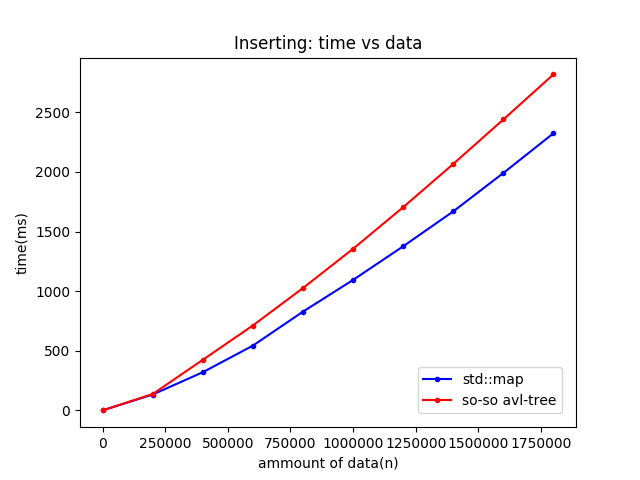
\includegraphics[width=\linewidth]{insert.png}
\end{center}
\begin{center}
    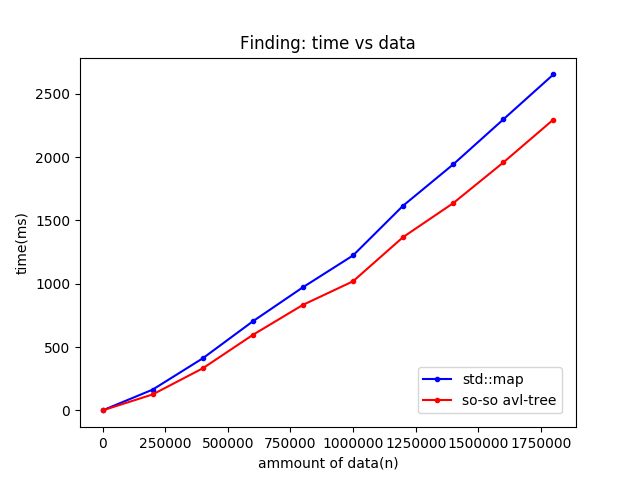
\includegraphics[width=\linewidth]{find.png}
\end{center}

\begin{center}
    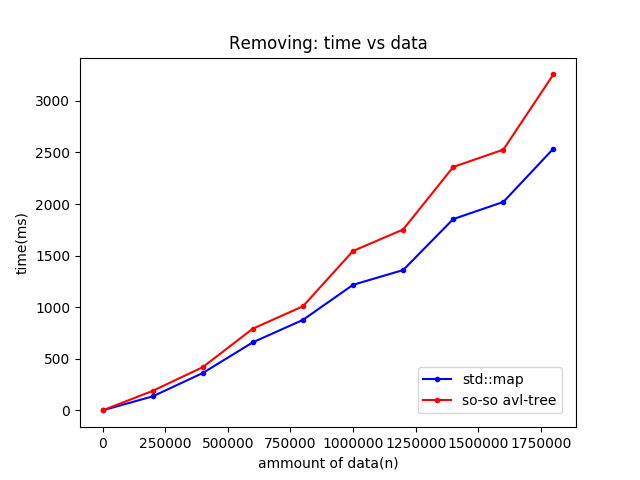
\includegraphics[width=\linewidth]{remove.png}
\end{center}

Не логарифмическая зависимость на графиках, по моему мнению, получается из-за довольно частых выделений/освобождений памяти на кучи, а это, как известно, не дешевая в плане времени операция.
К тому же графики имеют очень похожую форму, что говорит об асимптотически одинаковой скорости роста времени выполнения операций. А уж в \verb|stl| сомневаться не приходится.

\subsection*{Недочёты}

Программа работает не так быстро, как хотелось бы, хотя и прошла тестирование на чекере.

Узким местом, как выясняется, является пользовательский класс строк, что не удивительно. А именно считывание строки из потока. Из-за лишнних операций копирования и системных вызовов для выделения/возврата памяти программа замедляется.

Как решение можно предложить <<подглядеть>> как работают более удачные реализации строк и переделать/доделать свои строки с подобных методов.
Исправление нецелесообразно потому что лабораторная работа немного не про это.

\subsection*{Выводы}

Данная стркутура данных может быть применена как вспомогательная для решения большей задачи, например, в качестве словаря, множества, мультимножества(с доработками) и подобных этим абстрактным типам данных. Так же, весьма вероятно, в реализации простейших БД.

Первый раз реализовывать данную структуру было довольно сложно. Возможно, при повторном написании, получится сделать это быстрее и алгоритм получится оптимальнее.

Основные проблемы при написании возникли при леализации удаления из AVL-дерева из-за неполного понимания. Почему-то думалось, что балансировать нужно только дерево-родитель удаляемого узла, а, как оказалось, это не так.

Описать область применения реализованного алгоритма. Указать типовые
задачи, решаемые им. Оценить сложность программирования, кратко
описать возникшие проблемы при решении задачи. 

\end{document}

 
